\section{Masses}
We introduce \textit{masses} to simplify the function $\phi(i,j)$ in \cref{trans_spir,trans_spir_10}. We shorten the double product of these theorems to a much more elegant form using \textit{mass products}. We start by giving a number of definitions.

\begin{definition}[\cite{streams:degrees:suprema:2020}]{Weights and masses.}\hfill
	\begin{enumerate}
		\item We define a \textit{weight} as a tuple $\weight[a] := \tup{a_0,...,a_{n-1}}\in\Q^n$.
		\item We define the \textit{length} of a weight as $\abs{\weight[a]} := n$.
		\item We say that a weight $\weight[a]$ is \textit{positive} if $\weight[a]_i\geq0$ for all $i<\abs{\weight[a]}$.
		\item We say that a weight $\weight[a]$ is \textit{constant} if $\weight[a]_i = 0$ for all $i<\abs{\weight[a]}$. 
		\item We define a \textit{mass} as a tuple of positive weights $\mass = (\weight[a]_0,...,\weight[a]_{l-1})$.
		\item We define the \textit{length} of a mass as $\abs{\mass} := l$.
		\item We say that a mass $\mass$ is \textit{constant} if $\mass_i$ is constant for all $i<\abs{\weight[a]}$.
		\item We define $flat({\mass})$ as the concatination of all weights of $\mass$. For example $flat((\tup{1,2},\tup{3,4})) = \tup{1,2,3,4}$.
		\item We define the flattened length $\|\mass\|$ as the sum of the lengths of all weights in a mass: $$\|\mass\| := \sum_{i=0}^{\abs{\mass}}\;\abs{\mass_i}$$
	\end{enumerate}
\end{definition}

\begin{definition}[\cite{streams:degrees:suprema:2020}]{Weight and mass operations.}\label{product_displacement_definition}\\
	Let $f: \N \to \N$ be a natural function and $n\geq0$.
	\begin{enumerate}
		\item We define the rotation of a weight $\weight$ with $\abs{\weight} = l$ recursively:
		\begin{align*}
			\weight^{(0)} &:= \weight \\
			\weight^{(n+1)} &:= \tup{\weight_{l-1},\weight_{0},...,\weight_{l-2}}^{(n)}
		\end{align*}
		\item We define the rotation of a mass $\mass$ with $\abs{\mass}=l$ recursively:
		\begin{align*}
			\mass^{(0)} &:= \mass \\
			\mass^{(n+1)} &:= (\mass_{l-1},\mass_{0},...,\mass_{l-2})^{(n)}
		\end{align*}
		\item We define the \textit{scalar product} of a weight $\weight[a] = \tup{a_0,...,a_{q-1}}$ for some $q>0$ as:
		$$\weight[a]\odot f := \sum_{i=0}^{q-1} a_i*f(i)= a_0 * f(0) + a_0*f(1) + ... + a_{q-1}*f(q-1)$$
		\item We define the \textit{weight displacement} of a weight $\weight = \tup{a_0,...,a_{q-1}}$. Notice that we can write $n = qk + i$ for $i<q$ and $k\geq0$.
		\begin{align*}
			(\weight \oplus f): \N &\to \Q \\
			(\weight \oplus f)(n) &:= (\weight \oplus f)(qk + i) = a_i + f(qk + i)
		\end{align*}
		\item We define the \textit{mass product} of a mass $\mass$ recursively:
		\begin{align*}
			(\mass\otimes f): \N &\to \Q \\
			(\mass\otimes f)(0) &:= \mass_0 \odot f \\
			(\mass\otimes f)(n+1) &:= (\mass^{(1)} \otimes \shift{\abs{\mass_0}}{f})(n)
		\end{align*}
		\item We say that $(\weight \oplus (\mass \otimes f))$ is natural if $(\weight \oplus (\mass \otimes f))(n) \in \N$ for all $n \geq 0$ and likewise that $(\mass \otimes f)$ is natural if $(\mass \otimes f)(n) \in \N$ for all $n \geq 0$.
		\item We say that a weight $\weight$ is constant, if $\weight_i = 0$ for all $i<\abs{\weight}$.
		\item We say that a mass $\mass$ is constant, if al its weights are constant.
	\end{enumerate}
\end{definition}


\begin{example}
	We will show $\weight \oplus (\mass \otimes f)$ for the function $f(n) = 2n$, the mass $\mass := (\tup{0,1,\frac{1}{2}},\tup{3})$ and the weight $\weight := \tup{2,-8}$. Notice that $\weight \oplus (\mass \otimes f)$ is natural, even though the mass contains a fraction and the weight contains a negative number.
	\begin{figure}[H]
		\centering
		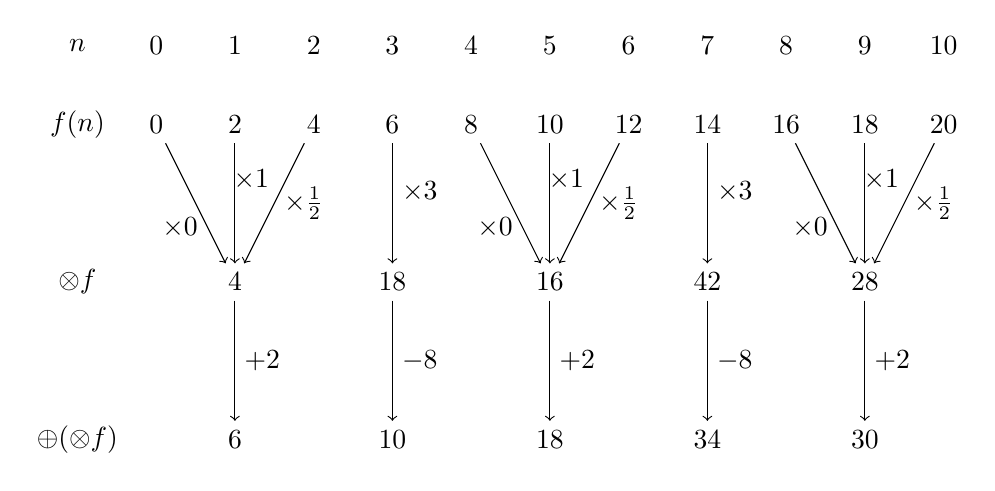
\begin{tikzpicture}[node distance=1.3cm]
			\node (n0) at (0,0) {$n$};
			\node (f0) at (0,-1) {$f(n)$};
			\node (m0) at (0,-3) {$\mass \otimes f$};
			\node (m0) at (0,-5) {$\weight \oplus (\mass \otimes f)$};

			\node (n1) at (1,0) {$0$};
			\node (n2) at (2,0) {$1$};
			\node (n3) at (3,0) {$2$};
			\node (n4) at (4,0) {$3$};
			\node (n5) at (5,0) {$4$};
			\node (n6) at (6,0) {$5$};
			\node (n7) at (7,0) {$6$};
			\node (n8) at (8,0) {$7$};
			\node (n9) at (9,0) {$8$};
			\node (n10) at (10,0) {$9$};
			\node (n11) at (11,0) {$10$};

			\node (f1) at (1,-1) {$0$};
			\node (f2) at (2,-1) {$2$};
			\node (f3) at (3,-1) {$4$};
			\node (f4) at (4,-1) {$6$};
			\node (f5) at (5,-1) {$8$};
			\node (f6) at (6,-1) {$10$};
			\node (f7) at (7,-1) {$12$};
			\node (f8) at (8,-1) {$14$};
			\node (f9) at (9,-1) {$16$};
			\node (f10) at (10,-1) {$18$};
			\node (f11) at (11,-1) {$20$};

			\node at (2,-3) (m1) {$4$};
			\node at (4,-3) (m2) {$18$};
			\node at (6,-3) (m3) {$16$};
			\node at (8,-3) (m4) {$42$};
			\node at (10,-3) (m5) {$28$};

			\draw[->] (f1) edge[pos=0.7] node[left] {$\times 0$} (m1);
			\draw[->] (f2) edge[pos=0.3] node[xshift=-4,right] {$\times 1$} (m1);
			\draw[->] (f3) edge node[right] {$\times \frac{1}{2}$} (m1);

			\draw[->] (f4) edge[pos=0.4] node[right] {$\times 3$} (m2);

			\draw[->] (f5) edge[pos=0.7] node[left] {$\times 0$} (m3);
			\draw[->] (f6) edge[pos=0.3] node[xshift=-4,right] {$\times 1$} (m3);
			\draw[->] (f7) edge node[right] {$\times \frac{1}{2}$} (m3);
			
			\draw[->] (f8) edge[pos=0.4] node[right] {$\times 3$} (m4);

			\draw[->] (f9) edge[pos=0.7] node[left] {$\times 0$} (m5);
			\draw[->] (f10) edge[pos=0.3] node[xshift=-4,right] {$\times 1$} (m5);
			\draw[->] (f11) edge node[right] {$\times \frac{1}{2}$} (m5);

			\node at (2,-5) (w1) {$6$};
			\node at (4,-5) (w2) {$10$};
			\node at (6,-5) (w3) {$18$};
			\node at (8,-5) (w4) {$34$};
			\node at (10,-5) (w5) {$30$};

			\draw[->] (m1) edge[] node[right] {$+ 2$} (w1);
			\draw[->] (m2) edge[] node[right] {$- 8$} (w2);
			\draw[->] (m3) edge[] node[right] {$+ 2$} (w3);
			\draw[->] (m4) edge[] node[right] {$- 8$} (w4);
			\draw[->] (m5) edge[] node[right] {$+ 2$} (w5);

		\end{tikzpicture}
		\caption{Example of a weight displacement applied to a mass product.}
		\label{fig:mass_prod}
	\end{figure}
\end{example}

\begin{lemma}[\cite{streams:degrees:squares:2015}]\label{single_weight_in_mass}
	Let $f: \N \to \N$ be a function. Let $\mass$ be a non-constant mass with $m:=\abs{\mass}$. Then there exists a list of non-constant weights $(\weight_i)_{i=0}^{m}$ such that:
	\begin{align*}
		\mass \otimes f = \fzip_m(g_0,g_1,\dots, g_{m-1}) \qquad\text{ where }\qquad g_i = ((\weight_i) \otimes f) \text{ for } i<m
	\end{align*}
	\begin{proof}
		We only show the basic idea.
		Let $\weight$ be a mass such that $\abs{\weight_i} = \|\mass[a]\|$ for all $i<m$.
		Define $s_l := \sum_{i=0}^{l}\abs{\mass[a]_i}$ for $l < m$.
		Define $\weight$ by
		\begin{align*}
			\mass[\b]_{i,s_j+h} := \quad
		\begin{cases}
			\mass[a]_{i,h}\quad &\text{if } j = i \\
			0 \quad &\text{if } j \neq i
		\end{cases}
		\qquad
		\text{ where } j<m \text{ and } h<\abs{\mass[a]_i}
		\end{align*}
		For example, if $\mass[a] = (\tup{1,2,3},\tup{1,2},\tup{0,1,0})$ then
		\begin{align*}
		\mass[b] = 
		\begin{pmatrix}
			\tup{1, 2, 3, 0, 0, 0, 0, 0}, \\
			\tup{0, 0, 0, 1, 2, 0, 0, 0}, \\
			\tup{0, 0, 0, 0, 0, 0, 1, 0}
		\end{pmatrix}
		\end{align*}
	\end{proof}
\end{lemma}

\begin{proposition}[\cite{streams:degrees:squares:2015}]\label{mass_spir}
	Let $f\in\spir$, let $\mass$ be a non-constant mass and $\weight$ a weight. Then we have:
	\begin{enumerate}
		\item $\weight \oplus f \in \spir$ if $\weight \oplus f$ is natural.
		\item If $\weight$ is positive and $(\weight)\otimes f$ is natural then $(\weight)\otimes f\in\spir$.
		\item $\mass\otimes f\in\spir$ if $\mass\otimes f$ is natural.
		\item $\weight\oplus(\mass\otimes f)\in\spir$ if $\weight\oplus(\mass\otimes f)$ is natural.
	\end{enumerate}
	\begin{proof}\hfill\\
		Let $q := \abs{\weight}$ and $l := \abs{\mass}$ be the lengths of the weight and mass respectively.
		\begin{enumerate}
			\item We show properties $(a)$ and $(b)$ of \cref{def_spir}.
			\begin{enumerate}
				\item 
				Let $m\geq 0$. Let $M := \min(\weight_0,\weight_1,\dots,\weight_{q-1})$. Because $f\in\spir$, we have, for some $N\geq0$, that $f(n) \geq \abs{M} + m$ for all $n \geq N$. Write $n = qk+i$ for $i<q$ and $k\geq0$.
				\begin{align*}
					(\weight \oplus f)(qk+i) = \weight_i + f(qk+i) \geq \weight_i + \abs{M} + m \geq m
				\end{align*}
				\item
				Let $m > 0$. Then because $f\in\spir$ we have $N\geq0,\;p>0$ such that for all $n\geq N$ we have $f(n+p)\equiv f(n) \mod m$. Let $\tilde{p} := q*p$. Write $n = qk+i$ for $i<q$ and $k\geq0$.
				\begin{gather*}
					(\weight \oplus f)(n) =
					(\weight \oplus f)(qk+i) = 
					\weight_i + f(qk+i) \equiv \\
					\weight_i + f(qk+i+pq) = 
					(\weight \oplus f)(n+\tilde{p}) \mod m
				\end{gather*}
			\end{enumerate}
			\item We show properties $(a)$ and $(b)$ of \cref{def_spir}. 
			We can say
			\begin{align*}
				\weight = \tup{\frac{a_0}{d},\frac{a_1}{d},\dots,\frac{a_{q-1}}{d}}
			\end{align*}
			where $a_j\geq0$ for all $j<q$ (because $\weight$ is positive) and $d>0$.
			Because the mass ``$(\weight)$'' only contains a single weight ``$\weight$'' we can easily give an explicit form of the mass product:
			\begin{align}
				((\weight) \otimes f)(n) &= 
				\weight \odot \shift{nq}{f} = \notag\\
				\sum_{i=0}^{q-1}\weight_i*(\shift{nq}{f})(i) &= 
				\sum_{i=0}^{q-1}\weight_i*f(nq+i) = \label{mass_spir.pf1} \\
				\sum_{i=0}^{q-1}\frac{a_i}{d}&*f(nq+i) \notag
			\end{align}
			\begin{enumerate}
				\item Let $m\geq0$, then by $f\in\spir$, we can find $N\geq0$ such that for all $n\geq N$ we have $f(n) \geq \frac{m}{b*q}$ where $b := \min(\frac{a_0}{d},\frac{a_1}{d},\dots,\frac{a_{q-1}}{d})$. Because $\weight$ is positive, we have for $n\geq N$, 
				\begin{align*}
					((\weight) \otimes f)(n) &\overset{\ref{mass_spir.pf1}}{=} 
					\sum_{i=0}^{q-1}\frac{a_i}{d}*f(nq+i) \geq \\
					\sum_{i=0}^{q-1}b*f(nq+i) &\geq
					\sum_{i=0}^{q-1}b*\frac{m}{b*q} =
					m
				\end{align*}
				\item Let $m>0$, then by $f\in\spir$, we can find $N\geq0,\; p>0$ such that: 
				\begin{align}
					f(n+p)\equiv f(n) \mod dm \label{mass_spir.pf2}
				\end{align}
				Then we have for $(k_i)\in(\Z)^{q}$ that:
				\begin{gather*}
					((\weight) \otimes f)(n) \overset{\ref{mass_spir.pf1}}{=}
					\sum_{i=0}^{q-1}\frac{a_i}{d}*f(nq+i) \overset{\ref{mass_spir.pf2}}{=} \\
					\sum_{i=0}^{q-1}\frac{a_i}{d}*(f(nq+i+pq) + k_imd) = \\
					\sum_{i=0}^{q-1}\frac{a_i}{d}*(f(nq+i+pq)) + \sum_{i=0}^{q-1}\frac{a_i}{d}*(k_imd) = \\
					\sum_{i=0}^{q-1}\frac{a_i}{d}*(f(nq+i+pq)) + \sum_{i=0}^{q-1}a_i(k_im) \equiv \\
					\sum_{i=0}^{q-1}\frac{a_i}{d}*(f(q(n+p)+i)) \overset{\ref{mass_spir.pf1}}{=}
					((\weight) \otimes f)(n+p) \mod m
				\end{gather*}
			\end{enumerate}
			\item Let $l := \abs{\mass}$, then we have by \cref{single_weight_in_mass} that:
			\begin{align*}
				\mass \otimes f = \fzip_{l}(g_0,g_1,\dots, g_{l-1}) \qquad\text{ where }\qquad g_i = ((\mass[b]_i) \otimes f) \text{ for } i<l
			\end{align*}
			for positive weights $\mass[b]_i$. In the previous item, we have seen that $g_i\in\spir$ for all $i<l$. The result follows from the fact that $\fzip$ is spiralling when all its arguments are spiralling as shown in \cref{\fzip_spir}.
			\item This follows from the first and third item.
		\end{enumerate}
	\end{proof}
\end{proposition}

\begin{lemma}{\cite{streams:degrees:squares:2015}}\label{f_transto_massprod}
	If $f\in\spir$ then $\fs{f} \geq \fs{\weight \oplus (\mass \otimes \shift{k}{f})}$ for any mass $\mass$, weight $\weight$ and $k\geq0$ if $\weight \oplus (\mass \otimes \shift{k}{f})$ is natural.
	\begin{proof}
		We give a sketch of this proof. 
		Let $f\in\spir$.
		Because $(\mass \otimes \shift{k}{f}) \in \spir$ by \cref{mass_spir}, we can seperately show that $\fs{f} \geq \mass \otimes \shift{k}{f}$ and $\fs{f} \geq \beta \oplus f$. We can also ignore the shift of $f$ because $\shift{k}{f}\in\spir$ by \cref{cp_spir} so that $\shift{k}{f} \equiv \fs{f}$ by \cref{simple_fs_facts}. \\
		\begin{stp}{$\fs{f} \geq \mass \otimes f$}
			We start by writing out the mass $\mass$.
			\begin{align*}
				\mass &= (\weight[a]_0,\weight[a]_1,..., \weight[a]_{l-1}) &\text{ where } \\
				\weight[a]_i &= \tup{\frac{a_{i,0}}{d_i},\frac{a_{i,1}}{d_i},...,\frac{a_{i,q_i}}{d_i}} &\text{ for } i < \abs{\mass} \text{ and where }
				q_i := \abs{\weight[a]_i}
			\end{align*}
			% We will construct a transducer $T = (Q,q_0,\delta,\lambda)$ that transduces $\fs{f}$ to $\mass \otimes \shift{k}{f}$.
			We will create three seperate transducers $T_1,T_2$ and $T_3$.
			\begin{enumerate}
				\item $T_1$ multiplies each value of $f$ by $a_{i,j}$ in a periodic way, such that:
				$$\fs{f} \geq_{T_1} \fs{n \mapsto (flat(\mass)_{n\mod \|\mass \|})*f(n)}$$
				\item $T_2$ adds the values together that belong to one weight. 
				\item $T_3$ divides the values of the resulting function by $d_i$.
			\end{enumerate}
		\end{stp}
		\begin{stp}{$\fs{f} \geq \weight \oplus f$}
			This follows from a similar construction as shown in \cref{trans_spir.pf3} combined with $T_3$ of the previous proof sketch. 
		\end{stp}
	\end{proof}
\end{lemma}

\begin{theorem}[\cite{streams:degrees:squares:2015}]\label{mass_product_spir}
	If $f\in\spir$, then $\fs{f} \geq \sigma$ if and only if $\sigma \equiv \fs{\weight\oplus(\mass\otimes \shift{k}{f})}$ for some integer $k\geq0$, a mass $\mass$ and a weight $\weight$.
	\begin{proof}{$(\implies)$}
		By \cref{trans_spir_10} we have that
		\begin{align*}
			\sigma &\equiv \prod_{i=0}^{\infty}\prod_{j=0}^{l-1} \s{10}^{\phi(i,j)}
			\qquad \text{ where } \qquad
			\phi(i,j) := \frac{f(N + li + j) - a_j}{z}
		\end{align*}
		for a number $l,z>0$ and $a_j\geq0$ for all $j<l$.
		Let $\weight := \tup{-\frac{a_0}{z},-\frac{a_1}{z},...,-\frac{a_{j-1}}{z}}$ and $\mass := ([z])$. Without loss of generality assume $N$ to be a multiple of $l$.
		For all $n\geq N$ write $n = N + il + j$ where $j<l$ and $i\geq 0$.

		\begin{align*}
			(\weight \oplus (\mass\otimes f))(n) &= 
			(\weight \oplus (\mass\otimes f))(N + il + j) = \\
			(\mass\otimes f)(N + il + j) - \frac{a_j}{z} &= 
			\frac{1}{z}*f(N + il + j) - \frac{a_j}{z} = \\
			\frac{f(N + il + j) }{z} - \frac{a_j}{z} &= 
			\frac{f(N + il + j) - a_j}{z} =
			\phi(i,j)
		\end{align*}

		We can use this derivation to write:

		\begin{gather*}
			\sigma \equiv \prod_{i=0}^{\infty}\prod_{j=0}^{l-1} \s{10}^{\phi(i,j)} \equiv  
			\bs{n}{0}{N}\cdot\prod_{i=0}^{\infty}\prod_{j=0}^{l-1} \s{10}^{(\weight \oplus (\mass \otimes f))(il + j)} \overset{\ref{basic_ineq}.\ref{basic_ineq.prepend}}{\equiv} \\ 
			\prod_{n=0}^{\infty} \s{10}^{(\weight \oplus (\mass \otimes f))(n)} = 
			\fs{\weight \oplus (\mass \otimes f)}
		\end{gather*}
		$(\impliedby)$
		If $\sigma \equiv \fs{\weight \oplus (\mass \otimes \shift{k}{f}})$, then by \cref{f_transto_massprod} we have $\fs{f} \geq \fs{\weight \otimes (\mass \otimes \shift{k}{f}}) \equiv \sigma$ thus by transitivity $\fs{f} \geq \sigma$.
	\end{proof}
\end{theorem}
